\documentclass[
border=10pt,
varwidth=24cm
]{standalone}

\usepackage[T1]{fontenc}
\usepackage[utf8]{inputenc}
\usepackage{lmodern}
\usepackage{array}
\usepackage{makecell}
\usepackage{amsmath}
\usepackage{amssymb}
\usepackage{tikz}

\usetikzlibrary{shapes.geometric}

\setlength{\parindent}{0pt}
\renewcommand{\arraystretch}{1.25}

% Adds padding inside every tabular cell, including cells containing
% nested tabulars and tikz pictures.
\setcellgapes{4pt}
\makegapedcells

% Cleaner paragraph columns: no paragraph indent and no stretched justification.
\newcolumntype{L}[1]{>{\raggedright\arraybackslash\setlength{\parindent}{0pt}}p{#1}}
\newcolumntype{C}[1]{>{\centering\arraybackslash\setlength{\parindent}{0pt}}p{#1}}

\newcommand{\tallyfive}{%
	\ensuremath{%
		\vcenter{\hbox{%
				\tikz[x=0.68ex, y=0.52ex]{
					% Balanced invisible box for centering
					\useasboundingbox (-0.5,-0.2) rectangle (3.5,4.2);
					
					% Four vertical tally marks
					\draw[line width=0.45pt, line cap=round] (0,0) -- (0,4);
					\draw[line width=0.45pt, line cap=round] (1,0) -- (1,4);
					\draw[line width=0.45pt, line cap=round] (2,0) -- (2,4);
					\draw[line width=0.45pt, line cap=round] (3,0) -- (3,4);
					
					% Diagonal crossing stroke
					\draw[line width=0.45pt, line cap=round] (-0.35,0.75) -- (3.35,3.25);
				}%
		}}%
	}%
}

\begin{document}
	
	\begin{center}
		{\Large\bfseries Cambridge -- Mathematics -- Stage 4 -- Paper 1}
	\end{center}
	
	\vspace{0.4cm}
	
	\begin{tabular}{|c|L{7.4cm}|c|L{3.6cm}|L{5.2cm}|}
		\hline
		\textbf{\#}
		& \multicolumn{1}{c|}{\textbf{Answer}}
		& \textbf{Marks}
		& \multicolumn{1}{c|}{\textbf{Part Marks}}
		& \multicolumn{1}{c|}{\textbf{Guidance}} \\
		\hline
		
		1(a) & 6324 & \centering 1 & & \\
		\hline
		
		1(b) & Thirteen thousand, seven hundred and forty two & \centering 1 & & Accept recognisable misspellings. \\
		\hline
		
		2 &
		\[
		\frac{1}{7}
		\qquad
		\frac{1}{5}
		\qquad
		\tikz[baseline=(x.base), scale=1.4, transform shape]{
			\node[draw,circle,inner sep=2pt] (x) {$\frac{1}{9}$};
		}
		\qquad
		\frac{1}{6}
		\]
		& \centering 1 & & Accept any clear indication. \\
		\hline
		
		3 &
		\begin{tabular}{|c|c|c|}
			\hline
			number of pets & tally & frequency \\
			\hline
			0--2 & $\tallyfive$ & 5 \\
			\hline
			3--5 & $\vert\vert\vert$ & 3 \\
			\hline
			6--8 & $\vert$ & 1 \\
			\hline
		\end{tabular}
		& \centering 2
		& Award 1 mark for any four or more boxes completed correctly.
		& Do not accept five lines for five in the tally column, e.g. $\vert\vert\vert\vert\vert$ \\
		\hline
		
		4 &
		\begin{tabular}{ccc}
			$-4$ & \fbox{$<$} & $3$ \\[1em]
			$9$ & \fbox{$>$} & $-2$
		\end{tabular}
		& \centering 1 & & Both answers correct for the mark. \\
		\hline
		
		5 & 41 and 36 & \centering 1 & & Both answers correct for the mark. \\
		\hline
		
		6 &
		\[
		60
		\qquad
		65
		\qquad
		70
		\qquad
		\tikz[baseline=(x.base), scale=1.2, transform shape]{
			\node[draw,circle,inner sep=2pt] (x) {$75$};
		}
		\qquad
		80
		\]
		& \centering 1 & & Accept any clear indication. \\
		\hline
		
		7 & Any two from 106, 116, 126
		& \centering 1
		&
		& Both answers correct for the mark. \\
		\hline
		
		8 &
		\begin{minipage}{7.2cm}
			\centering
			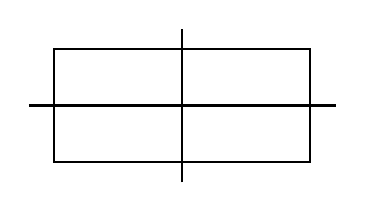
\begin{tikzpicture}[scale=0.65]
				% Rectangle
				\draw[thick] (0,0) rectangle (5,2.2);
				
				% Lines of symmetry
				\draw[thick] (-0.5,1.1) -- (5.5,1.1);
				\draw[thick] (2.5,-0.4) -- (2.5,2.6);
			\end{tikzpicture}
		\end{minipage}
		& \centering 1
		&
		& Both lines drawn as shown.
		
		Accept slight inaccuracies as long as intention is clear. \\
		\hline
		
		9 &
		\begin{minipage}{7.2cm}
			\centering
			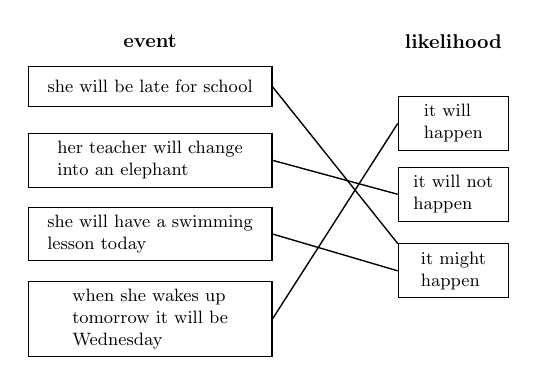
\begin{tikzpicture}[scale=0.72, every node/.style={font=\small, transform shape}]
				% Headings
				\node[font=\bfseries] at (1.9,5.25) {event};
				\node[font=\bfseries] at (7.25,5.25) {likelihood};
				
				% Event boxes
				\node[
				draw,
				minimum width=4.3cm,
				minimum height=0.70cm,
				align=left,
				inner sep=4pt
				] (e1) at (1.9,4.45)
				{she will be late for school};
				
				\node[
				draw,
				minimum width=4.3cm,
				minimum height=0.90cm,
				align=left,
				inner sep=4pt
				] (e2) at (1.9,3.15)
				{her teacher will change\\into an elephant};
				
				\node[
				draw,
				minimum width=4.3cm,
				minimum height=0.90cm,
				align=left,
				inner sep=4pt
				] (e3) at (1.9,1.85)
				{she will have a swimming\\lesson today};
				
				\node[
				draw,
				minimum width=4.3cm,
				minimum height=1.20cm,
				align=left,
				inner sep=4pt
				] (e4) at (1.9,0.35)
				{when she wakes up\\tomorrow it will be\\Wednesday};
				
				% Likelihood boxes
				\node[
				draw,
				minimum width=1.95cm,
				minimum height=0.85cm,
				align=left,
				inner sep=4pt
				] (l1) at (7.25,3.80)
				{it will\\happen};
				
				\node[
				draw,
				minimum width=1.95cm,
				minimum height=0.85cm,
				align=left,
				inner sep=4pt
				] (l2) at (7.25,2.55)
				{it will not\\happen};
				
				\node[
				draw,
				minimum width=1.95cm,
				minimum height=0.85cm,
				align=left,
				inner sep=4pt
				] (l3) at (7.25,1.20)
				{it might\\happen};
				
				% Matching lines
				\draw[line width=0.5pt] (e1.east) -- (l3.north west);
				\draw[line width=0.5pt] (e2.east) -- (l2.west);
				\draw[line width=0.5pt] (e3.east) -- (l3.west);
				\draw[line width=0.5pt] (e4.east) -- (l1.west);
			\end{tikzpicture}
		\end{minipage}
		& \centering 2
		& Award 1 mark for any two or three correct lines.
		& Accept any clear indication. \\
		\hline
		
		10 &
		\begin{minipage}{7.2cm}
			\centering
			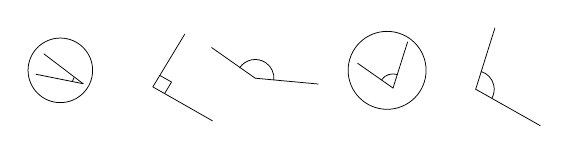
\begin{tikzpicture}[
				scale=0.5,
				line cap=round,
				line join=round,
				line width=0.275pt
				]
				% Option 1
				\begin{scope}[shift={(0,0)}]
					\draw (0,0) circle (0.82);
					\coordinate (V1) at (0.58,-0.34);
					\draw (-0.42,0.42) -- (V1);
					\draw (-0.62,-0.10) -- (V1);
					\draw (V1) ++(146:0.28)
					arc[start angle=146,end angle=168,radius=0.28];
				\end{scope}
				
				% Option 2
				\begin{scope}[shift={(2.35,-0.42)}, scale=0.88]
					\coordinate (V2) at (0,0);
					\coordinate (A2) at (0.92,1.52);
					\coordinate (B2) at (1.72,-0.98);
					\draw (V2) -- (A2);
					\draw (V2) -- (B2);
					\coordinate (P2) at (0.20,0.33);
					\coordinate (Q2) at (0.34,-0.19);
					\coordinate (R2) at (0.54,0.14);
					\draw (P2) -- (R2) -- (Q2);
				\end{scope}
				
				% Option 3
				\begin{scope}[shift={(4.95,-0.20)}, scale=0.82]
					\coordinate (V3) at (0,0);
					\draw (V3) -- (-1.35,0.95);
					\draw (V3) -- (1.95,-0.18);
					\draw (V3) ++(146:0.58)
					arc[start angle=146,end angle=-5,radius=0.58];
				\end{scope}
				
				% Option 4
				\begin{scope}[shift={(8.20,0)}]
					\draw (0.1,0) circle (0.99);
					\coordinate (V4) at (0.25,-0.45);
					\draw (V4) -- (-0.65,0.18);
					\draw (V4) -- (0.62,0.72);
					\draw (V4) ++(145:0.36)
					arc[start angle=145,end angle=72,radius=0.36];
				\end{scope}
				
				% Option 5
				\begin{scope}[shift={(10.55,-0.48)}, scale=0.84]
					\coordinate (V5) at (0,0);
					\draw (V5) -- (0.58,1.85);
					\draw (V5) -- (1.95,-1.10);
					\draw (V5) ++(73:0.56)
					arc[start angle=73,end angle=-29,radius=0.56];
				\end{scope}
			\end{tikzpicture}
		\end{minipage}
		& \centering 1
		&
		& Both answers correct for the mark.
		
		Accept any clear indication. \\
		\hline
		
		11 &
		\begin{minipage}{7.2cm}
			\centering
			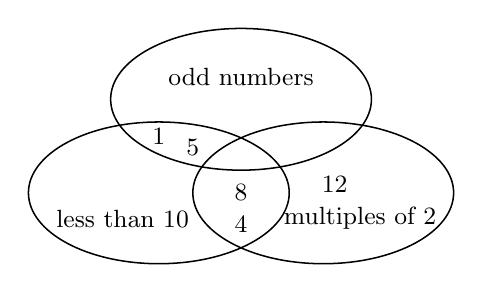
\begin{tikzpicture}[
				scale=0.72,
				line cap=round,
				line join=round,
				every node/.style={font=\small}
				]
				% Ellipses
				\draw[line width=0.55pt] (0,1.65) ellipse (2.30 and 1.25);
				\draw[line width=0.55pt] (-1.45,0) ellipse (2.30 and 1.25);
				\draw[line width=0.55pt] (1.45,0) ellipse (2.30 and 1.25);
				
				% Set labels
				\node at (0,2.05) {odd numbers};
				\node at (-2.09,-0.45) {less than 10};
				\node at (2.1,-0.45) {multiples of 2};
				
				% Numbers
				\node at (-1.45,0.99) {1};
				\node at (-0.85,0.8) {5};
				\node at (0,0) {8};
				\node at (0,-0.55) {4};
				\node at (1.65,0.15) {12};
			\end{tikzpicture}
		\end{minipage}
		& \centering 2
		& Award 1 mark for any three or four correctly placed with no numbers repeated.
		& \\
		\hline
		
		12 & 24 (cm$^2$)
		& \centering 1
		&
		& \\
		\hline
		
		13 &
		\[
		\begin{array}{cc}
			1 \div 6 = 6
			&
			\tikz[baseline=(x.base), scale=1.2, transform shape]{
				\node[draw,ellipse,inner sep=4pt] (x) {$1 \div 6 = \dfrac{1}{6}$};
			}
			\\[1em]
			6 \div 1 = 6
			&
			6 \div 1 = \dfrac{1}{6}
		\end{array}
		\]
		& \centering 1
		&
		& Accept any clear indication. \\
		\hline
		
		14 &
		134 indicated with an explanation to show that 134 is not odd, e.g.
		
		it has an even digit in the ones place.
		
		\textbf{or}
		
		it can be divided exactly by 2 (so it is even)
		& \centering 1
		&
		& \\
		\hline
		
		15 &
		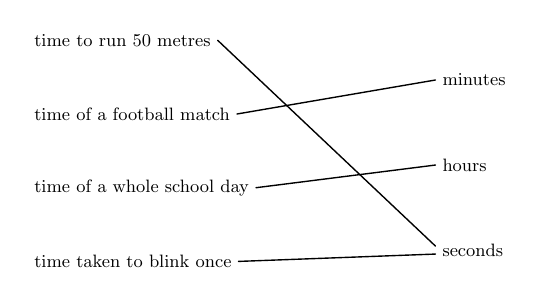
\begin{tikzpicture}[
			scale=0.72,
			every node/.style={font=\small, transform shape},
			line cap=round,
			line join=round
			]
			% Left labels
			\node[anchor=west, align=left] (a1) at (0,3.9) {time to run 50 metres};
			\node[anchor=west, align=left] (a2) at (0,2.6) {time of a football match};
			\node[anchor=west, align=left] (a3) at (0,1.3) {time of a whole school day};
			\node[anchor=west, align=left] (a4) at (0,0.0) {time taken to blink once};
			
			% Right labels
			\node[anchor=west] (b1) at (7.2,3.2) {minutes};
			\node[anchor=west] (b2) at (7.2,1.7) {hours};
			\node[anchor=west] (b3) at (7.2,0.2) {seconds};
			
			% Matching lines
			\draw[line width=0.5pt] (a1.east) -- ([yshift=2pt]b3.west);
			\draw[line width=0.5pt] (a2.east) -- (b1.west);
			\draw[line width=0.5pt] (a3.east) -- (b2.west);
			\draw[line width=0.5pt] (a4.east) -- ([yshift=-2pt]b3.west);
		\end{tikzpicture}
		& \centering 2
		& Award 1 mark for any two or three correct lines.
		& Accept any clear indication. \\
		\hline
		
		16 &
		\begin{tabular}{|c|}
			\hline
			\textbf{direction Eva walks along} \\
			\textbf{each path} \\
			\hline
			north \\
			\hline
			east or E \\
			\hline
			north or N \\
			\hline
			northeast or NE \\
			\hline
			southeast or SE \\
			\hline
		\end{tabular}
		& \centering 1
		&
		& All four correct directions for the mark.
		
		Accept recognisable misspellings. \\
		\hline
		
		17 &
		Accept answers in the range of \(16\)--\(18\) \((\mathrm{cm}^2)\) inclusive, e.g. \(17\) \((\mathrm{cm}^2)\)
		& \centering 1
		&
		& \\
		\hline
		
		18 & 105 (hours) & \centering 1 & & \\
		\hline
		
		19 &
		\begin{tabular}{ccc}
			\(\dfrac{8}{15}\) & \fbox{\(\,<\,\)} & \(\dfrac{3}{5}\) \\[0.35cm]
			\(\dfrac{8}{20}\) & \fbox{\(\,=\,\)} & \(\dfrac{4}{10}\)
		\end{tabular}
		& \centering 1
		&
		& Both answers correct for the mark. \\
		\hline
		
		20 & 13 (boxes) & \centering 1 & & Do not accept 13 r 4 \\
		\hline
		
		21 &
		An explanation that states that the total number of children who chose music (as a favourite hobby) is 21 \((9+12)\) and the total number of children who chose reading (as a favourite hobby) is 22 \((13+9)\) (so Naomi is wrong).
		
		\vspace{0.2cm}
		Accept there is one more child who chose reading than music.
		
		\vspace{0.2cm}
		Accept any correct numerical comparison between \(9+12\) and \(13+9\).
		
		\vspace{0.2cm}
		Do not accept any explanation without numerical evidence.
		& \centering 1
		&
		& \\
		\hline
		
		22 &
		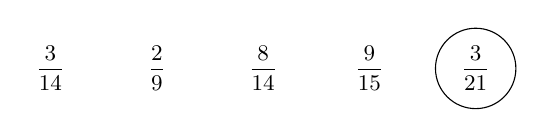
\begin{tikzpicture}[scale=0.9, every node/.style={font=\small, transform shape}]
			\node at (0,0) {\(\dfrac{3}{14}\)};
			\node at (1.5,0) {\(\dfrac{2}{9}\)};
			\node at (3.0,0) {\(\dfrac{8}{14}\)};
			\node at (4.5,0) {\(\dfrac{9}{15}\)};
			\node[draw, circle, inner sep=4pt] at (6.0,0) {\(\dfrac{3}{21}\)};
		\end{tikzpicture}
		& \centering 1
		&
		& Accept any clear indication. \\
		\hline
		
		23 &
		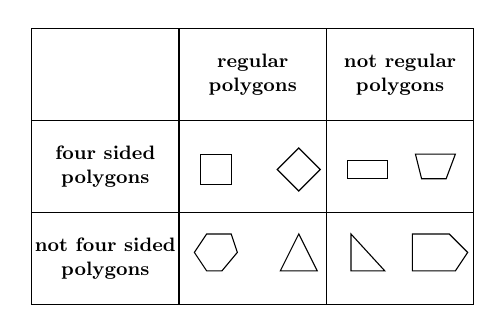
\begin{tikzpicture}[
			scale=0.78,
			baseline=(current bounding box.north),
			every node/.style={font=\small, transform shape}
			]
			% Table grid
			\draw (0,0) rectangle (7.2,4.5);
			\draw (2.4,0) -- (2.4,4.5);
			\draw (4.8,0) -- (4.8,4.5);
			\draw (0,1.5) -- (7.2,1.5);
			\draw (0,3.0) -- (7.2,3.0);
			
			% Column headings
			\node[align=center, font=\bfseries\small] at (3.6,3.75) {regular\\polygons};
			\node[align=center, font=\bfseries\small] at (6.0,3.75) {not regular\\polygons};
			
			% Row headings
			\node[align=center, font=\bfseries\small] at (1.2,2.25) {four sided\\polygons};
			\node[align=center, font=\bfseries\small] at (1.2,0.75) {not four sided\\polygons};
			
			% Four sided regular polygons
			\draw (2.75,1.95) rectangle (3.25,2.45);
			\draw (4.00,2.20) -- (4.35,2.55) -- (4.70,2.20) -- (4.35,1.85) -- cycle;
			
			% Four sided not regular polygons
			\draw (5.15,2.05) rectangle (5.80,2.35);
			\draw (6.25,2.45) -- (6.90,2.45) -- (6.75,2.05) -- (6.35,2.05) -- cycle;
			
			% Not four sided regular polygons
			\draw (3.10,0.55) -- (3.35,0.85) -- (3.25,1.15) -- (2.85,1.15) -- (2.65,0.85) -- (2.85,0.55) -- cycle;
			\draw (4.05,0.55) -- (4.35,1.15) -- (4.65,0.55) -- cycle;
			
			% Not four sided not regular polygons
			\draw (5.20,0.55) -- (5.20,1.15) -- (5.75,0.55) -- cycle;
			\draw (6.20,0.55) -- (6.90,0.55) -- (7.10,0.85) -- (6.80,1.15) -- (6.20,1.15) -- cycle;
		\end{tikzpicture}
		& \centering 2
		& Award 1 mark for each correct pair of headings.
		& Accept the word `shapes' instead of polygons.
		
		For the mark the pairs in rows or columns must use consistent terminology, e.g. do not accept regular polygons and not regular shapes. \\
		\hline
		
		24 &
		\begin{minipage}{7.2cm}
			$(2, 7)$ and $(6, 7)$
			
			\vspace{0.2cm}
			\centering
			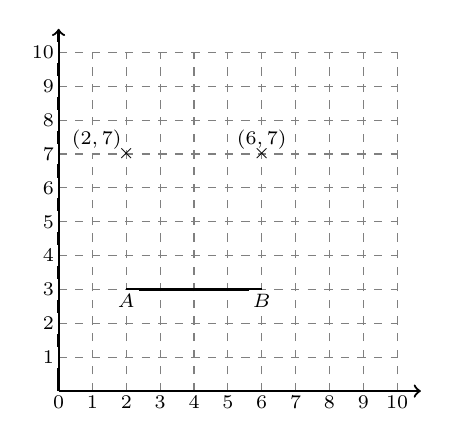
\begin{tikzpicture}[
				scale=0.43,
				every node/.style={
					font=\scriptsize,
					fill=white,
					inner sep=1.5pt
				}
				]
				% Grid
				\draw[dashed, gray] (0,0) grid (10,10);
				
				% Axes
				\draw[->, thick] (0,0) -- (10.7,0);
				\draw[->, thick] (0,0) -- (0,10.7);
				
				% Axis labels
				\foreach \x in {0,1,...,10}
				\node[below] at (\x,0) {\x};
				\foreach \y in {1,2,...,10}
				\node[left] at (0,\y) {\y};
				
				% Original segment
				\draw[thick] (2,3) -- (6,3);
				\node[below] at (2,3) {$A$};
				\node[below] at (6,3) {$B$};
				
				% Answer points
				\node[above left] at (2,7) {$(2, 7)$};
				\node[fill=none, inner sep=0pt] at (2,7) {$\times$};

				\node[above] at (6,7) {$(6, 7)$};
				\node[fill=none, inner sep=0pt] at (6,7) {$\times$};
			\end{tikzpicture}
		\end{minipage}
		& \centering 1
		&
		& Accept coordinates written on the grid.
		
		Do not accept points without coordinates on the grid. \\
		\hline
		
	\end{tabular}
	
\end{document}